\documentclass[12pt,a4paper]{article}
\usepackage[utf8]{inputenc}
\usepackage[english]{babel}
\usepackage{amsmath}
\usepackage{amsfonts}
\usepackage{amssymb}
\usepackage{graphicx}
\usepackage{fullpage}
\usepackage{hyperref}

\usepackage{titling}
\newcommand{\subtitle}[1]{%
  \posttitle{%
    \par\end{center}
    \begin{center}\large#1\end{center}
    \vskip0.5em}%
}

\author{Michele Carignani, Alessandro Lenzi}
\title{Community discovery in Milan}
\subtitle{project for the course of Distributed Enabling Platforms}

\makeindex

\begin{document}

\maketitle
\tableofcontents

\begin{abstract}
The aim of the project is to analyze and then visualize telecommunication data
in order to discover real-world communities basing on the number of mobile telecommunications (calls and text messages) 
between different geographical areas. We design and implemented 
a parallel computation as a pipeline of
map reduce jobs onto the Hadoop distributed computation
framewor and environment\footnote{http://hadoop.apache.org/}.
In sections \ref{thedataset} and \ref{ds_analysis} of this report, we describe the original dataset
and analyze its properties. Then in section \ref{aggregation}
we explain how we rearranged the data in
order to reduce the noise and improve the tractability and robustness of the
community discovery phase. Sections \ref{approaches} and \ref{mcl} will then
briefly describe two different approaches for community discovery
(finding strongly connected components and markovian clustering)
and in detail describe strategy and implementation of the latter which has
proved to give more significant results.
Finally section \ref{results} will collect results and conclusion of the developed project.
All the implementation code for the project can be found in this
\href{''https://github.com/michele-carignani/hadoop-markov-clustering/''}{online repository}.
\end{abstract}

%% Dataset and analysis
\section{Dataset}
\label{thedataset}

\paragraph{The dataset} on which the analysis has been developed is an aggregated log of mobile phone
calls and short text messages with their geographical source and destination points.
The dataset is composed by several textual files, each one containing information of one specific day
within the observation period of two months (november and december 2013).

\paragraph{In each file,} a row describes the \textbf{connection strength between two geographical areas} in the Province of Milan (Italy) during a time period of 10 minutes within the day.
The definition, given by the provider of the dataset, of connection strength between two areas is: a decimal value proportional to the number of calls and sms sent from one area to another one.

\paragraph{The grid} Geographic areas are identified by a logical a grid of $10.000$ squared areas (with area $10.000m^2$)
% todo: controllare numero
identified by an integer number $i \in [0, 9999]$ where the
$ i / 100 $ and $ i \% 100 $ are respectively the  
x and y coordinates of the node.

To give an example, the dataset is compose of $62$ text files, named like \verb!2013-11-01.txt!, containing lines with the format:

\begin{verbatim}
timestamp \t sourceNode	\t 	destNode
\end{verbatim}

where \verb!timestamp! is the time in milliseconds describing the first millisecond of the period described, \verb!sourceNode! is an integer describing the source and \verb!destNode! is an integer identifying the destination areas of call and messages within the logical grid.

Summing up, the dataset describes several \footnote{precisely there are 8784 graphs, one for each 10-minutes interval within the observation period of 61 days.} \textbf{directed weighted graphs over
the nodes of the geopgraphical grid}.
Records where the values is zero are not listed. Each file has a size between
3 and 6 GBs and the total size of the dataset is around 450GB.

\section{Data distributions analysis}
\label{ds_analysis}




\section{Model}
In our model, we started by considering what is a community. In our interpretation of this word,
we defined a community as a set of individuals with close relationship, meaning high probability to interact or to have someone in common with whom they interact.

Since we're dealing with mobile telecommunications, the idea is that a community can be identified by the frequency of calls and text messages between members belonging
to the same community.

The idea behind this approach is that, since we're searching for a community, we don't care about their size (i.e. the probability for an individual to be in a certain "community"), 
but only the probability that two geographical areas (and thus, in our model, their inhabitants) can be correlated by their calls.

The assumptions that we made are:
\begin{itemize}
\item People are related to some zones more strongly, meaning that an individual 
has an higher probability of staying in certain zones (for example, near his work place or near his home) than in random places
in the area taken into consideration. This allows to relate calls from certain geographical zones to some people.
\item People call more often other people belonging to their community.
\item Is not of major interest who is colling whom, since we only care about the existance of a ''binding'' between the two individuals.
\item A person may belong to several communities, however depending on the day and on the time of the call, the probability of communicating with a certain community changes.
As an example, during work hours it is more probable that calls will be addressed to people related to the working activity, while outside it will involve more probably family and friends
\footnote{Similarly, Telco operators have been known to distinguish between business traffic and residential traffic.}.
\end{itemize}

As it is possible to see, using the strengths as an indicator "as they are", zones with an higher population or with an higher concentration of calls could obfuscate the behaviour of less populated zones, justifying why the probabilistic approach has been followed.

We can think of the initial dataset as composed of several graphs, one for each 10 minutes slots, in which the strengths connecting two areas are seen as weights of the arcs connecting them. We denote this strength, which is given in the
dataset and is proportional to the amount of calls directed from a certain zone to another, with $S_{i,j}$. 
Of course, whenever $S_{i,j}$ is not given in the dataset for a given ten-minutes graph, we will assume that its value is 0, and thus that no calls from $i$ to $j$ have been performed.

The probability of one call between grid $i$ and grid $j$ is thus assumed by us to be: 
$$
P_{i,j} = P\{call(i,j)\} = \frac{S_{i,j}}{\sum_{j}{}{S_{i,j}}}
$$
where $P\{call(i,j)\}$ indicates the probability of the event \emph{call(i,j)}, meaning that a call in grid $i$ is performed and addressed to grid $j$.

However notice that using a single 10 minutes graph is not particularly significative, as it could be possible to have spikes of traffics in some zones due to unpredictable events (i.e. a car accident, a demonstration, an exibition and so on) that we don't want to take into account for individuating stable communities.
So, to get more realistic results and to deal with the very high level of noise in the dataset,
we decided to gather and average the strength of interaction between couples of nodes in several 10-minutes periods
considering a semantically meaningful aggregation in time (not alway contiguous, e.g. we aggregating all working hours in working days), in which we assumed that the behaviour of commmunities would be more or less the same.
\label{AVGPG}
We called these aggregations \emph{average probability graphs}, in which nodes are cells in the grid of our dataset, arcs represent interactions and, for each of them, the weight represents the average probability that such an interaction is established.

To be more formal, let $A$ be the set of arcs of the initial dataset and $E_{id} \subseteq E$ be the set of arcs belonging to aggregation $id$ composed of $k$ 10-minutes intervals, then the weight $w_{id}(e)=\widehat{P_{i,j}}$ of an arc $e=(i,j)$ of the average graph for aggregation period $id$ will be 
$$
w_{id}(e) = \frac{\sum_{\substack{e' \in E_{id}}} w(e')}{k}
$$

In the following, we will show how we performed the calculation of these \emph{aggregated probability graphs} and how we used the produced results in order to find communities in the Milan Area.

%% How aggregated graphs are generated
\section{Data aggregation}
\label{aggregation}
In our model, we dealt with interactions between different nodes in the considered area, rescaling them and considering them as probabilities.
However, often the little aggregation time lead to very noisy datasets, among which it was difficult to operate achieving meaningful results.

So, to get more realistic results and to deal with the very high level of noise in the dataset,
we decided to gather and average the strength of interaction between couples of nodes in several 10-minutes periods
considering a semantically meaningful aggregation in time (not alway contiguous, e.g. we aggregated all monday
mornings periods).

To achieve this, we developed a procedure composed by two consecutive logical map reduce computations executable with the Hadoop environment.
The input of the \emph{Time Aggregation} phase is the raw dataset, while the output is a graph of probabilities of interaction between zones of the considered area
over a certain period of interest.
Here follows the pseudo-code of the map and reduce operations.

\begin{verbatim}
FilterMap(key, value):
// input takes in input all dataset files
// implementeted in aggregated_graphs.FilterMapper.java
  d = parse(value)
  if (d.timestamp belongs_to interesting_period)
  	k = (interesting_period,d.sourceNode,d.destNode)
  	v = d.value
    emit(k, v)

AverageReduce(key,values):
// implemented in aggregated_graphs.AverageReducer.java
  sum = count = 0
  for v in values:
  	sum += v
  	count++
  (id,num,source,dest) = parse(key)
  avg = sum / num
  emit((id,source),(dest,value))

IdentityMap(key, value):
  emit(key, value)

ProbabilityReduce(key, values):
  sum = 0
  a_list = []
  for v in values:
    (dest, weight) = parse(v)
    sum += weight
  	a_list.append((dest,weight))

  for a in a_list:
    emit((key.src, a.dest), a.weight / sum)
\end{verbatim}

\subsection{Implementation details}

\paragraph{Disk usage}: During the initial executions, our testing environment
could complete the aggregation of large periods (that means,
aggregations including many 10-minutes intervals) because of full
disk utilization. 
While passing the filtered edges from the mappers to the reducers
writing the splits (around 800 file splits produced by
as many mappers) the disk was filled up.
To overcome this issues, we used several approaches:
\begin{enumerate}
\item \textbf{Combiners} a combiner has been defined to shrink the first map output size. The combiner performs a sum over all strengths in the same aggregation period and, of course, with same source and destination. 
The output of the combiner is a graph for each aggregation period in which the strength is the sum of all strength.
This solution, for an aggregation with size of n slots, could reduce the output of each map task up to $1/n$ of the original size without the combiner.
\item \textbf{GZip} another approach that we tried, and thereafter discarded, was to use GZip as compression codec for data going out of the map. From experimental results, we noticed that this approach, altough not providing enough benefits
to cope with disk utilization issues, slowed down our computation significantly.
\item \textbf{Change in split size} thanks to the combiner, the biggest is the number of time slots gathered in a single aggregation, the biggest is the shrinking in data. 
Therefore, we tried to increase the size of the splits to be given to a single map task to exploit this reduction. We progressively increased split size from 128Mb to 1GB and then to contain a single whole file, which was not splittable.
However, we noticed that this method, while decreasing the efficiency in the cluster utilization (as only fewer processing units could be used together) and in the completion time of this phase, was still not enough to cope with our disk issues.
\item \textbf{Divide et impera} the latest, and best approach to solve the disk space issue, was to change the logic in the driver. What was previously the first map-reduce phase, has been decomposed into several little map-reduce phases, each one taking a parametric
chunk of the initial data. This led to benefits from the point of view of disk usage, of completion time and of cluster utilization.
\end{enumerate}




\section{Communities discovery approaches}
\label{approaches}

Once the aggregated graph is produced (as list of weighted edges) is time to compute
the communities (i.e. the clusters) over it.

Two different approaches were developed and tested. 
As we will see, the second will give the
expected results, while the first will fail.

\subsection{Tarjan Connected Components algorithm}
%todo: explain cuts
Defining the communities as connected components onto the graph\footnote{A connected component
in a graph $A = (N,E)$ is a subset of nodes $A' \in A$  s.t. each node in A' is connected to 
all the other nodes in A' 
%% todo: more formal definition?
}, the first idea was to apply Tarjan's algorithm for connected components, whose pseudo code is in \ref{alg:tarjan}.


In our initial approach, a mere visit, ordered on the arc identifier (i.e. \texttt{for i = 0 to 10000 do strongconnect(i)}) was performed. This visit, though executed with different cuts over the probability of the arcs, evidenced
a strong bias of the order of visit on the found strongly connected components.
As an example, with a cut on probability 0.005, a huge SCC is found, containing almost all nodes. Only few nodes remain
outside this CFC, and some small aggregations can be found between them.
So our second step has been achieving a visiting strategy consistent with the effective traffic measured during the day.
To do so, we used the measurements of the total activity of grids in order to establish a visiting order to be 
followed during the procedure.
\begin{figure}
\begin{verbatim}
input: graph G = (V, E)
output: set of strongly connected components (sets of vertices)
index := 0
S := empty
for each v in V do
	if (v.index is undefined) then
		strongconnect(v)
		
function strongconnect(v)
v.index := index
v.lowlink := index
index := index + 1
S.push(v)
for each (v, w) in E do
	if (w.index is undefined) then
		strongconnect(w)
		v.lowlink := min(v.lowlink, w.lowlink)
		else if (w is in S) then
			v.lowlink := min(v.lowlink, w.index)
if (v.lowlink = v.index) then
	start a new strongly connected component
	do
		w := S.pop()
		add w to current strongly connected component
	until (w = v)
	output the current strongly connected component
end function
\end{verbatim}
\caption{Tarjan Strongly Connected Components algorithm}
\label{alg:tarjan}
\end{figure}
We performed the following attempts and different visits on our graph:
\begin{enumerate}
\item Nodes visited for increasing outgoing hourly traffic, with arcs selected with increasing probability. 
\item Nodes visited for decreasing outgoing hourly traffic, with arcs ordered with increasing probability.
\item Nodes visited for decreasing outgoing hourly traffic, with arcs ordered with decreasing probability.
\item Nodes visited for increasing outgoing hourly traffic, with arcs ordered with decreasing probability.
\end{enumerate}
\begin{figure}
\centering
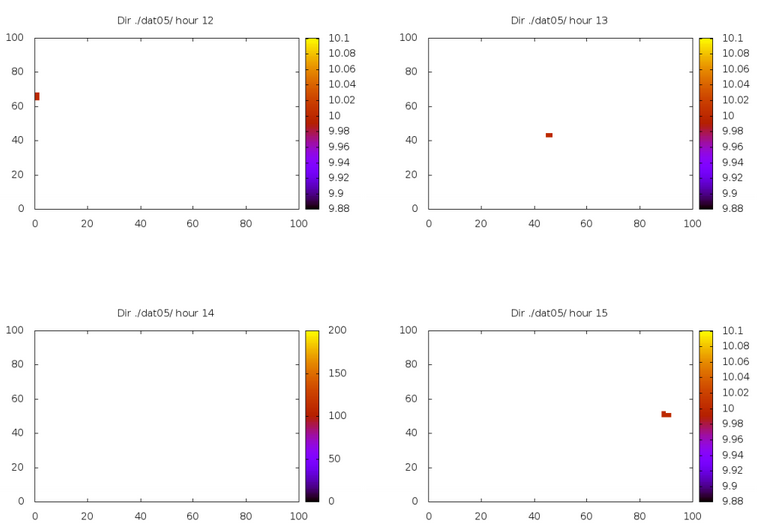
\includegraphics[scale=0.5]{tarjanscc.png}
\caption{Strongly connected components found with Tarjan Algorithm.From left to right, top to bottom the hours considered are 12, 13, 14, 15.
The visit has been performed with increasing hourly traffic and arcs selected with increasing probability. 
The cut has been performed at value 0.05.}
\label{fig:tarjan1}
\end{figure}
\begin{figure}
\centering
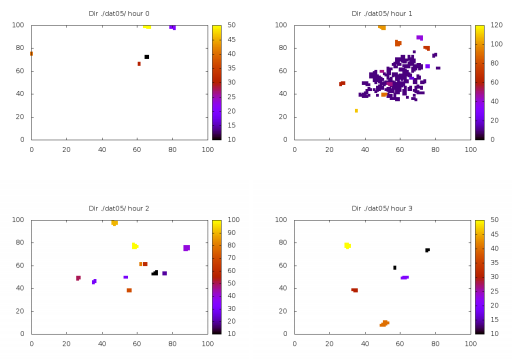
\includegraphics[scale=0.6]{tarjanscc2.png}
\caption{Stronglu connected components found with Tarjan Algorithms. From left to right, top to bottom the hours considered are 0, 1, 2 and 3.
The visits have been performed with increasing hourly traffic and arcs selected with increasing probability.
Cut performed at value 0.05}
\label{fig:tarjan2}
\end{figure}

The image \ref{fig:tarjan1} shows the found strongly connected components in the most trafficated hours 
of the analysis. As it is possible to notice by looking to \ref{fig:analysis}, in fact, during
these hours arcs values are very concentrated near the mean, and thus most of them will be cutted out, making
most of the strongly connected components to disappear in the most trafficated hours of the day.
The results are slightly better in less trafficated hours as shown in \ref{fig:tarjan2}, in which the variance is higher and thus a wider number
of arcs will "save himself" from the performed cutting.
In other attempts, we tried to modify the threshold so that it would save more arcs for the computation,
but we have not been able to find an appropriate threshold leading to a large enough number of clusters
and with an acceptable size.\\
In fact, in most cases, a too low threshold led to few huge connected components whilst too high led to few and very small
connected components.\\
The approach described above, in our opinion, could not lead to the desired results because of two reasons:
\begin{itemize}
\item First, the visiting order, though more meaningful, was still establishing a bias in the search of the components because
of the "paths" eliminated by the original Tarjan algorithm
\item and second, the "static" threshold did not adapt well to changing traffic along the days.
\end{itemize}
To overcome this issues, we decided to implement a small variation of the Tarjan SCC algorithm, in which visited nodes not
becoming part of a strongly connected component could be visited again while searching for others, thus increasing the
complexity of the algorithm but with the advantage of reducing the visit ordering bias.
\\
The other modification that we implemented was that of percentile-based cuts. In this approach, for every hour, the probability
distribution has been calculated and only arc probabilities in a certain percentile have been held, while the others
have been cutted as it was done before with a "static" threshold. This allows for a more fine-grained cutting, allowing
to keep more arcs also in more trafficated hours of the day.

\begin{figure}
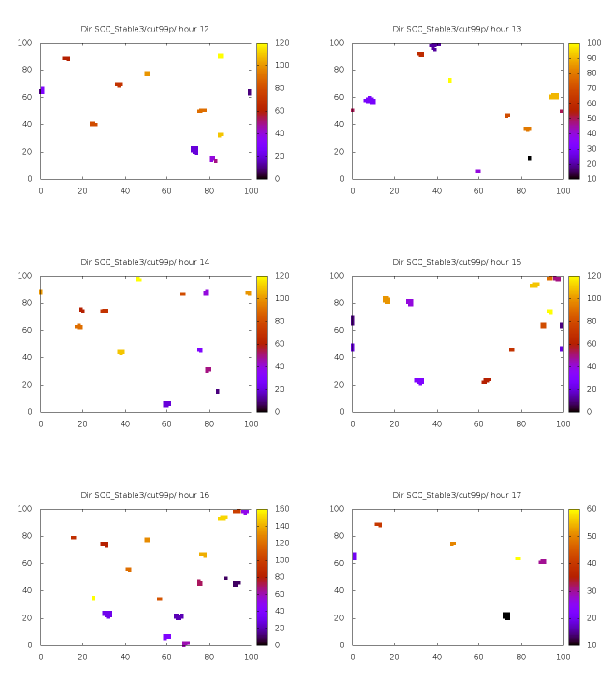
\includegraphics[scale=0.8]{tarjan3.png}
\caption{Strongly connected components found cutting at the 99-th percentile. Hours depicted are, from left to right and from top to bottom, 12-17.}
\label{fig:tarjan3}
\end{figure}

In \ref{fig:tarjan3} this modified algorithm has been tried with a cut on the 99-th precentile. In the plot
for the SCC found in this case, it is possible to see that most of them are geographically localized (as we expected),
but still their size is very small. \\
However, only few components were able to "survive" across several hours, and are mostly localized in the outskirts 
of the city. \\
Other attempts have been made to find suitable strongly connected components, but also small modification in percentiles
led either to very noise results (with almost all zones in the same component) or to empty results. 
From this approach, we understood that
\begin{enumerate}
\item Very high cuts are needed, because of the high connectivity degree of the graph
\item The statistics of arcs probabilities, however, seem to indicate the existance of zones calling themselves significantly more frequently than others.
\item Visiting strategy has a very strong bias, and probably never considering twice the same arc could lead to eliminate some interesting strongly connected components
\item The number of components is almost always lower than the expected one, however they are uniformly spreaded along the space taken into consideration
\item In different hours, the components vary in their positions, possibly indicating different users behaviours in different hours
\item Specially during hours in which we expected less traffic, components tend to move towards the outskirts, possibly denoting clusters belonging to small towns near Milan
\item The found components are not stable during consecutive hours but they appear and disappear. In the beginning we thought this was due to the "static" cut, but the reproposition
of this behaviour with the percentile denotes that the reason must be either a very noisy dataset or high variation in the users behaviours during the day.
\end{enumerate}

As previously said in Chapter 2, all of this research led us to the conclusion that the best approach was to find a sort of "average behaviour" to analyse and
to move to a different approach, in which communities are seen as clusters. 
To do so, we chose the \emph{Markov Clustering} algorithm, which is known in litterature for the purpose of finding communities in graphs.


For a more complete dissertation on what we did using this approach for discovering communities, we invite you to refer to the attacched file \texttt{CfcSuGrafiOrari.pdf}, in Italian.

\subsection{Markov Clustering}

We then looked at a diffferent approach: Markov Clustering based on the Markov Clustering Algorithm by Stijn van Dongen\footnote{\url{http://micans.org/mcl/}}.

The idea was to reduce noise and emphasize relations in a more structured way
by multiplying the adjancy matrix of the graph by itself until the number of
non-null elements in each row is very low (reduce the number of edges) and with
values probability weight close to 1 (taking the most probable connections).

Therefore, the pseudocode of the general algorithm is:
\begin{figure}
\begin{verbatim}
   G is a graph
   r = 4
   set M_1 to be the matrix of random walks on G

   while (change) {
      M_2 =  M_1 * M_1
      M_1 =  inflation(M_2)
      change   = difference(M_1, M_2)
   }

   set CLUSTERING as the components of M_1
\end{verbatim}
\caption{Markov Clustering pseudocode}
\end{figure}

The algorithm is based on the assumption that $G$ is a graph
were edges are weighted with probabilities and the sum
of all edges exiting a node is 1. Thus the adjacency matrix
of the graph is stochastic by rows.

The matrix can be therefore seen as the matrix of probabilities
of transitioning from a state to another state in
a Markov Process, also called random walk matrix.

The Markovian Clustering Algorithm simulates fluxes within the
graphs and calculates, with n iterations, the probabilities of going in
n steps from each node to another one. Taking this simulation to the limit
(or better, to a appropriate approximation of the limit) identifies
the most probable destinations of the flux from each node.

\section{Looking for communities with Markov Clustering}
\label{mcl}

In the next sections we explain in details the implementation of the
different phases of MCL.

\subsection{Convergency loop}
This loop is repeated a number of times, until the convergence is reached or the maximum
number of loops is executed.
The convergency loop is composed of 3 phases:
\begin{enumerate}
\item Matrix Multiplication, in which the current stochastic matrix is multiplied by itself
\item Matrix Inflation, an operation used to fasten convergency and whose aim and implementation will be explained in the following
\item Matrix Convergence Checker, used to compare achieved values with the previous ones.
\end{enumerate}

Given the matrix $A$ of step $i$, matrix $A'$ output of step $i+1$ has reached the convergency
if the following holds:
$$
\forall i,j . |A_{i,j} - A'_{i,j}| < \epsilon
$$ 
where $\epsilon$ is a parameter of the computation.
In order to minimize occupied space, to fasten convergency and to avoid pathological
cases to lead to "false convergency" (i.e. if the Markov Chain represented by the
matrix is characterized by periodicity), we decided to avoid matrix power method 
and to make the convergency loop proced as the Fibonacci series, meaning
that at step $i$ the matrix calculated in the loop will be $A^{fib(i)}$.
In the following, we will explain in detail the various phases in this convergency
loop.

\subsection{Matrix multiplication}
The first phase of the loop is \textbf{Matrix Multiplication}. For this part, we followed different
approaches for the implementation as map-reduce computations. While the first two approaches
revealed themselves to be very effective when dealing with dummy data using for the tests,
when real data was fetched both showed significant drawbacks that induced us to search for
a third solution, that is the one actually implemented in the delivered project.

Several implementations needed to be developed and tested in order to
achieve feasibility (onto the given environment) and improve performances.

\subsubsection{One step map-reduce}
In the beginning, we started by thinking that a simple approach could be producing all
couples to be multiplied of the two matrices with an appropriate index.\footnote{This algorithm
has been readapted and implemented starting from this website: http://importantfish.com/one-step-matrix-multiplication-with-hadoop/}
In this case, we have two different Map functions for two different files. To implement this in Map-Reduce, we exploited
the MultipleInputs function provided by the framework indicating for the two matrices a different mapper able
to emit different values.
The "first" matrix is fetched to the \texttt{OneStepRowMap} of fig. \ref{fig:onestepMaps} while the second to the \texttt{ColumnMap} of the same figure. In the pseudocode, there's no consideration for cases in which the value is 0, since the
matrix is already memorized neglecting null values.
The output of both mappers is fetched to \texttt{OneStepReduce} of fig. \ref{fig:onestepReduce}.
\begin{figure}
\begin{verbatim}
OneStepRowMap(key, value):
    for k = 1 to N:
        emit((value.row, k), ('A', value.column, value.probability))
OneStepColumnMap(key, value)
    for k = 1 to N:
        emit((k, value.column), ('B', value.row, value.probability))
\end{verbatim}
\caption{RowMap and ColumnMap used in the One-Step matrix multiplication algorithm. N is the size of the matrix, which is assumed to be square.}
\label{fig:onestep}
\end{figure}

\begin{figure}
\begin{verbatim}
OneStepReduce(key, values):
    A[N] = {j: a_ij for (x, j, a_ij) in values if x == A}
    B[N] = {j: b_jk for (x, j, b_jk) in values if x == B}
    result = 0
    for j = 1 to N:
        result += hash_A[j] * hash_B[j]
    emit(key, result)
\end{verbatim}
\caption{OneStepReduce used in the One-Step matrix multiplication algorithm. The key represents a single element in the matrix}
\label{fig:onestepReduce}
\end{figure}
As it is possible to understand very easily, with actual data this kind of implementation could not
work, since for every matrix element $N=10^4$ elements are emitted. Elements
are themselves $10^8$, making the total number of couples emitted by the mapper $10^12$.

Approximating the couple (key, value) with the size of its biggest component-
the double precision floating point probability values taking 128 bits on 64 word
machines - we would have needed a total memory of 128TB, which is much larger than
our enviroment total memory space, making impossible to carry on the computation
for dense matrices.


This implementation produced on our test environment a runtime expection
because of the memory being empty.

In fact, the Mappers writes their output in files but before this is put onto memory
and, since for every matrix element the mapper emits $N=10^4$ elements, and the elements
are themselves $10^8$ the total number of couples (key, value) written in memory
by the mappers to then be written on HDSF to be passed to the reducer was $10^{12}$.

Approximating the couple (key, value) with the size of its biggest component-
the double precision floating point probability values taking 128 bits on 64 word
machines - we would have needed a total memory of 128TB, which would be much larger than
our enviroment total memory space.

\subsubsection{Two step map-reduce}
The second approach has been the one of decomposing the computation further, trying to avoid
the explosion of data emitted caused by the algorithm discussed before.
In this approach, we have two map reduce steps.\footnote{Once again, this algorithmhas been readapted and implemented
following the post available at http://importantfish.com/two-step-matrix-multiplication-with-hadoop/}

In the mappers shown in fig. \ref{fig:twoStep1Map} used in the first step - again we distinguished between the two matrices using MultipleInputs - rows and columns values are emitted using their index as key.
In the reducer in fig. \ref{fig:twoStep1Reducer}the values of the row and column received are distinguished using the "A" and "B" flags. Subsequently,
every row value is multiplied for every column value, and this multiplied values are emitted using as key
the position of the value of the output matrix to which they will contribute. %todo: cec improbabol inglisc
\begin{figure}
\begin{verbatim}
TwoStepRowMap(key, value):
    emit(value.row, ("A", value.column, value.probability))

TwoStepColumnMap(key, value):
    emit(value.column, ("B", value.row, value.probability))
\end{verbatim}
\caption{Mappers used in the first phase of the two-step matrix multiplication algorithm.}
\label{fig:twoStep1Map}
\end{figure}
\begin{figure}
\begin{verbatim}
reduce(key, values):
    list_A = {(i, a_ij) for (M, i, a_ij) in values if M == "A"}
    list_B = {(k, b_jk) for (M, k, b_jk) in values if M == "B"}
    for (i, a_ij) in list_A:
        for (k, b_jk) in list_B:
            emit((i, k), a_ij*b_jk)
\end{verbatim}
\caption{Reducer used in the first phase of the two-step matrix multiplication algorithm.}
\label{fig:twoStep1Reducer}
\end{figure}

The second map-reduce phase of this algorithm implements the identity function in the mapper, and sums up all
multiplicated values for a certain value of the final matrix in the reducer shown in fig. \ref{fig:twoStep2Reducer}

\begin{figure}
\begin{verbatim}
reduce(key, values):
    result = 0
    for value in values:
        result += value
    emit(key, result)
\end{verbatim}
\caption{Reducer used in the second phase of the two-step matrix multiplication algorithm, summing up al row-by-column values concurring in its calculation.}
\label{fig:twoStep2Reducer}
\end{figure}
Even though this algorithm is way more optimized with respect to the previous one, since it also avoids to emit intermediate couples for possibly null values, it has reveled to be very slow in practice. This is due, in our opinion, to the need
of writing intermediate data between the two steps of the job in HDFS, which slows down computation significantly.

Also in this case some disk problems could arise, because once again, in the worst case, the intermediate data between the two steps is in general $1/2$ of the one emitted by the mapepr in the previous case, making once again
this algorithm unfeasible for the data we were dealing with.
We will se how we solved this problem, by decomposing in smaller parts the input matrix, in the following part.

\subsubsection{Block-wise}
With this approach, to cope with the problems related to the disk, we divided the matrix into several blocks.
Blocks have been enforced to have always the same size, and the approach discussed below has been used.

Let $\mathbf{A}$ and $\mathbf{B}$ be two NxN matrix, and let $p$ be the number of row/column partitions given
as input parameter, meaning that $p^2$ blocks will be produced for each matrix. As an example, we can decompose
A as follows:
$$
\mathbf{A} =
\begin{bmatrix}
    \mathbf{A_{1,1}} & \mathbf{A_{1,2}} & ... & \mathbf{A_{1,p}} \\
    \mathbf{A_{2,1}} & ... & ... \\
    ... \\
    \mathbf{A_{p,1}} & ... & ... & \mathbf{A_{p,p}}
\end{bmatrix}
$$
Now let both $\mathbf{A}$ and $\mathbf{B}$ be decomposed as explained before, we can calculate a single block $\mathbf{C_{i,j}}$
of the matrix $\mathbf{C} = \mathbf{A} x \mathbf{B}$ as follows:
$$
    \mathbf{C_{i,j}} = \sum_{k=1}^{p} \mathbf{A_{i,k}} \times \mathbf{B_{k, j}}
$$
This approach allows, with a sufficient decomposition, to prevent any problem related to disk usage and, in the meanwhile,
produced with some test matrices a way faster computation in the latest implementation.
In fact, the inner multiplication - to be clear, the one between two blocks in the decomposition of the matrices given
as input of this phase - has been implemented in three different way:
\begin{enumerate}
\item In the first case, we tried the (now promising) one-step matrix multiplication algorithm proposed above. However also in this case the output of the mapper revealed himself as huge, as also for a $1/10$-th partition of the matrix (with 1000 values) this approach would produce $10^9$ values, which is certainly a manageable size but still big enough to slow down the computation significantly, specially when considering the huge number of such multiplications to perform to calculate the whole $\mathbf{C}.$
\item In the second case, to be honest merely for the sake of completeness, we tried also to plug-in as multiplication module the two-step matrix multiplication algorithm. As it could have been foreseen, also this approach - though faster than the previous one - was still not fast enough to meet our requirements.
\item The third case, which is the one used in the final project, revealed himself to be the best both in terms of space and in completion time. This algorithm merely multiplies two blocks using the good old $O(n^3)$ sequential row-by-column matrix multiplication.
\end{enumerate}

As it is possible to understand, the approach that we finally decided to follow is very efficient for several resons.
Consider the case in which the number of partitions is 10, thus achieving 100 blocks for each of the two multiplied matrices.
The blocks will contain, in a worst case approximaton, $10^6$ doubles, meaning that a block multiplication will fit in memory and thus result in better performances, since also the output of each block-by-block multiplication will have size of approximately 32MB each, considering also the indexes.

Notice that this values, on our environment, allow to multiply several blocks in parallel, leading to a very good utilization
factor of the machines and nice results in terms of completion time.
The detailed implementation of this part is discussed thoroughly in \ref{blockmul}.

\subsubsection{Block-wise multiplication implementation}
\label{blockmul}
We wanted to develop, in this part, an highly parametrized system so to finely tune our computation to make it faster,
given that this is the biggest contributor to the completion time of the convergency loop, which is executed also several times.
For this reason, a module, called BlockWiseMatrixMultiplication has been developed, with the aim of allowing parametrized execution.

This module, which implements the \texttt{Tool} interface of the Hadoop framework, can be executed specifying the number
of blocks of the final matrix $\mathbf{C_{i,j}}$ to be executed in parallel. It takes also in input the directory containing
the two input matrices splitted in blocks and the directory in which the results must be written. Partitions are 
calculated automatically scanning the blocks by horizontal coordinates (by row) and then by column.

For each block multiplication scheduled by this very simple partitioner, a new thread is forked, which is responsible
for starting and monitoring all the jobs (running in parallel) consisting of the multiplications $\mathbf{A_{i,k}} \times \mathbf{B_{k,j}}$ needed to calculate $\mathbf{C_{i,j}}$.

In order for them to run in parallel, we used the \texttt{JobControl} class of the Hadoop framework, which allows to
schedule parallel jobs (and also to define dependencies between jobs). For every output block $\mathbf{C_{i,j}}$ $p$ 
multiplications of the original matrix blocks are performed as independent jobs running in parallel. 
These jobs consist of a single map-reduce phase, in which the mappers (as usual, one for the row and one for the column exploiting MultipleInputs) of fig. \ref{fig:blockwisemap} take care of "joining" and labelling the two blocks to be multiplied.
In the reducer, the whole blocks are gathered and saved in a matrix, which is then multiplied before the final values
are written in output, as it is possible to see in fig. \ref{fig:blockwisereduce}.
In the reducer, a slight optimization has been achieved by memorizing the second matrix (accessed k times) by column
and not by row, to avoid jumps in memory and to exploit caches and memory in the best possible way.

\begin{figure}
\begin{verbatim}
BlockRowMapper(key, value):
    emit(
      value.blockVerticalIndex, 
      ('A',value.row_id,value.column_id, value.probability)
    )

BlockColumnMapper(key, value):
    emit(value.blockHorizontalIndex, ('B', value.row_id, value.column_id, value.probability))
\end{verbatim}
\caption{Mappers used in the block-wise matrix multiplication. The block $\mathbf{A_{i,k}}$ is managed by BlockRowMapper, while $\mathbf{B_{k,j}}$ by BlockColumnMapper. This names are given merely for consinstency wrt. previous algorithms} 
\label{fig:blockwisemap}
\end{figure}

\begin{figure}
\begin{verbatim}
MatrixMultiplicationReducer(key, values):
    A[N/p][N/p]
    B[N/p][N/p]
    for v in values
        if v.label = 'A'
            A[v.row_id][v.col_id] = v.probability
        else
            B[v.col_id][v.row_id] = v.probability
    for i in [1, N/p]
        for j in [1, N/p]
            sum = 0
            for k in [1, N/p]
                sum += A[i][k]*B[j][k]
            if sum > 0
                emit((i,j), sum)
\end{verbatim}
\caption{Reducer used in the block-wise matrix multiplication. It performs the usual row-by-column matrix multiplication algorithm. N is the size of the matrix, p is the number of splits}
\label{fig:blockwisereduce}
\end{figure}
The second job needed to finally compute $\mathbf{C_{i,j}}$ is the one performing the sum over all partial matrices produced before, in order to achieve the real values in the computed block.
This job has, in its configuration, the horizontal and vertical coordinates $i$ and $j$ of the output block. In its mapper of fig. \ref{fig:blocksummap}, it aggregates by block row id and block column id the elements, so that they can be subsequently summed in the reducer as of fig. \ref{fig:blocksumreduce}.
This job is dependant of the previous ones, thus starts as soon as all the input data needed has been produced.
\begin{figure}
\begin{verbatim}
BlockSumMapper(key, value):
    emit((value.row_id, value.col_id), value.probability)
\end{verbatim}
\caption{The map function used to perform the sum over all partial matrices $\mathbf{A_{i,k}} \times \mathbf{B_{k,j}}$ and thus to calculate $\mathbf{C_{i,j}}$}
\label{fig:blocksummap}
\end{figure}
\begin{figure}
\begin{verbatim}
BlockSumReducer(key, values):
    blockIdX = get(block.horizontal_coordinates)
    blockIdY = get(block.vertical_coordinates)
    sum = 0
    for v in values
        sum += v
    emit((blockIdX, blockIdY, key.row_id, key._column_id), sum)
\end{verbatim}
\caption{The reduce function used to calculate the sum over single values in a position of the block and which writes out the final block.}
\label{fig:blocksumreduce}
\end{figure}
The thread forked and running the JobControl containing all such "individual block" jobs running in parallel, is checked periodically by another thread for completion. When this phase terminates, another set of blocks of parametric size
is calculated and the related multiplications are run.
This approach of not running everything in parallel has been pursued in order to avoid disk space issues and also to be 
able to avoid too much contention in the system.
From experimental results, in fact, we were able to verify that the matrix multiplication can be made very fast by dividing
initial matrices in 25 blocks and using partitions of size from 5 (corresponding thus to an entire row).

The drawback of this approach is that some others modules - for decomposing and recomposing the matrix - must be executed, as we wanted our procedure not to affect the final matrix representation.

These modules implementation is discussed in \ref{splitter} and \ref{recombiner}.
Finally, the behaviour of a single block multiplication is sketched in fig. \ref{fig:blockmultiplicationsketch}, while
the comprehensive driver of the matrix multiplication procedure that we finally adopted is illustrated in fig. \ref{fig:matrixmultiplicationsketch}, and its source code can be seen on %todo: insert link.

\begin{figure}
\centering
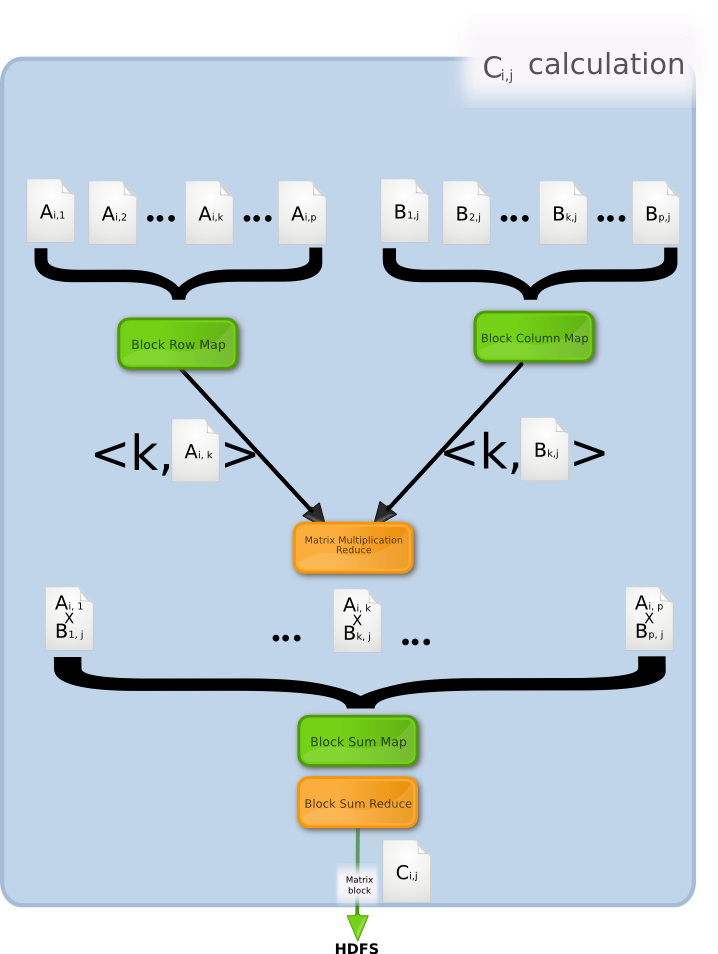
\includegraphics[scale=0.7]{blockmultiplication.png}
\caption{Procedure followed to calculate a single $\mathbf{C_{i,j}}$.}
\label{fig:blockmultiplicationsketch}
\end{figure}

\begin{figure}
\centering
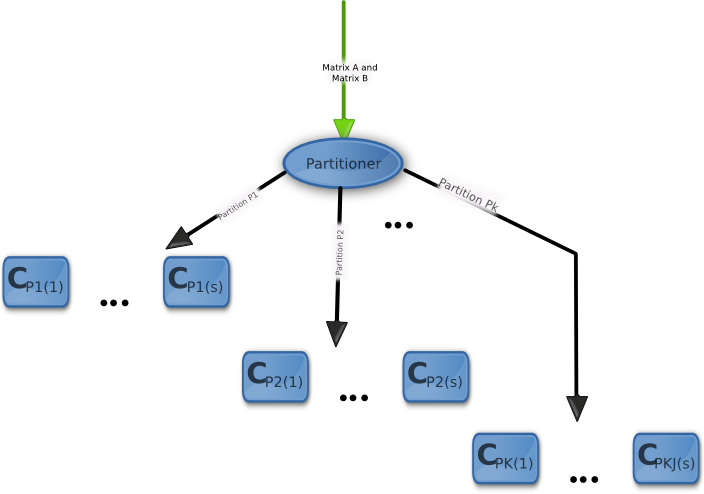
\includegraphics[scale=0.7]{matrixmultiplication.png}
\caption{Whole matrix multiplication procedure in a block-wise fashion. S blocks of the matrix are calculated
in parallel, while the others wait for the completion of the previous ones before going on.
In the image, s is the maximum size of the partition, k is assumed as the number of partitions and Pi(n) is a function
returning the index of the n-th block in partition Pi.In the image, the blue blocks titled after the matrix block they are used to compute represent the calculation shown in fig. \ref{fig:blockmultiplicationsketch}}
\label{fig:matrixmultiplicationsketch}
\end{figure}

\subsection{Inflation}

After multiplying the matrix by the last precedently computed, we apply a strategy
called inflation in order to enlarge differences between elements in a row.
Using the algorithm author words: ''richests get richer, poorests get poorer''.
In fact our main porpouse is to emphasize strong connections and to hide
weak ones.

For each row, we compute the sum of all r-th powers of its elements.
Then we recompute the element i,j as
$$ a_{i,j} = \frac{a_{ij}^r} {\sum_{k=0..N} a_{ik}^r}$$


\subsection{Convergency}
The convergency checker is a simple map-reduce job. The mapper takes as input the two matrices, the one 
newly calculated and the one calculated in the previous step. 
Then it emits the probability for a certain value using as key the coordinates of the probability, which
in this case are represented by a couple of coordinates, the former referring to the block and the latter to the
relative position inside the block.

In the reducer, these two values are subtracte and their difference confronted against the threshold. Whenever 
the difference is bigger than the threshold, a \texttt{Counter}, provided by the Hadoop framework is incremented by one,
making the job (whose output is always empty) return the number of non converged values.
Finally the driver checks for the value of this counter as soon as the job finishes, to check if a new convergency iteration
has to be executed or if the matrix has converged.

For what regards the speed of convergency, we observed that in the beginning values tend to converge very fast, approximately halving at every iteration for the first 10-15 iterations. Thereafter, the number of non-converging values continues to decrease
but in a more slow fashion, arriving from 16th iteration on to decrease only of an order of 10 values for iteration.
However, in these iterations the number of non-converged values is already very small, usually about 2000, and thus 
represents only the 0.2\% of the total values.
For this reason, we decided that 20 iterations were enough for our problem.

\subsection{Matrix splitter}
\label{splitter}
\subsection{Matrix recombiner}
\label{recombiner}
\subsection{Driver}
The driver for the Markov Clustering algorithm that we implemented is thus composed of several phases.
It takes as input parameters the following values:
\begin{enumerate}
\item \textbf{Input folder}, containing a probability matrix to be seen as a Markov Chain
\item \textbf{Output folder}, where the results will be written
\item \textbf{Maximum number of iterations}, the maximum number of convergency loops to perform before stopping
\item \textbf{Number of workers}, parameter used to decide how many matrix blocks multiplications should be computed in parallel.
\end{enumerate}
Starting from this phase, in the beginning the matrix is pre-processed and divided in blocks. The matrix is replicated on two different directories, that will be fetched in input to the first matrix multiplication phase.

The matrix multiplication phase works operating on 3 directories. It rotates in modulo 3 wrt to iteration number, taking the first two as input and the last as output folder.
However, the matrix multiplication writes on a temporary "inflate" directory. It will be the Inflation module responsible for filling the output dir of the phase with the ultimate result.
The convergency phase, instead, as previously explained, doesn't write down any information on the disk but merely exploits hadoop counters to understand the number of non converged values existing in the matrix.
Finally, when the matrix converges or the number of maximum iterations has been reached, the matrix is recomposed and written in the output directory.

A sketch depicting the behaviour of the whole pipeline that we developed can be seen in fig. \ref{fig:completepipeline}
\newpage
\begin{figure}
\centering
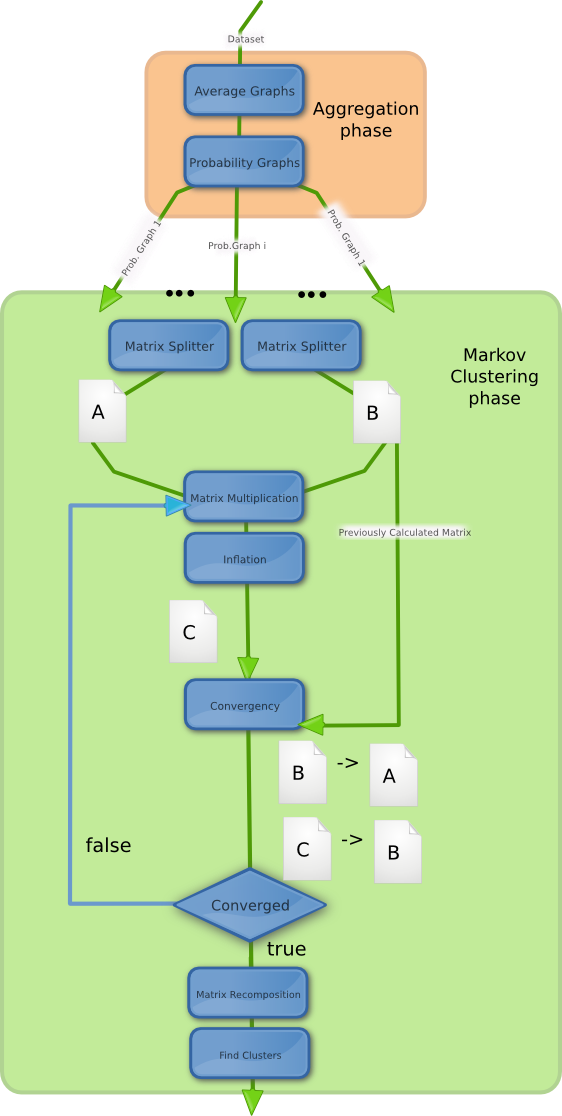
\includegraphics[scale=0.7]{completepipeline.png}
\label{fig:completepipeline}
\end{figure}
\newpage
\subsection{Finding clusters}
By the definition given in the original paper, given a matrix
multiplied until convergency is reached, the clusters are
identified as disjoint components in the graph, that means
a partition of the set of nodes such that there are no edges
linking two nodes which belong two different subsets in the partition.

In the  final matrix actually, values that are not 0 are 1 or tend to 1
and since this is stochastic matrix, this means that for each row
only one value is different from zero.

This, in turn, means that our aim of reduce the graph density toward
a linear number of edges, w.r.t the number of nodes, were  actually reached.

In this scenario, it is much more probable to discover disjoint compoments
of the graph, i.e clusters, i.e communities.

We implemented the last module of our application, the DisjointComponentVisit
class, as a visit
of the graph able of recognizing the different disjoint componets, which
defines and uses three main actions:
\begin{itemize}
    \item \verb!new_component()! creates a new subset of nodes,
    \item \verb!merge_components(c1,c2)! merges two subsets into one,
    \item \verb!add_to(n,c)! add a node to a subset.
\end{itemize}

The module, cycles over all edges in the result files, looks
for the components containing the head and the tail of the egde,
the in case they are the same it continues. If the head and tail
belong to different component, they are merged into one.
If one of the two nodes does not belong to any components, it is
added  to the component of the other one (in case none of them 
are contained in any components, a new component is created and both
are added to it).

We used the Java class \verb!java.util.TreeSet! to implement
the components which assures logarithmic time for
the operations of adding a new element and testing if an element
is contained. 

Since the expected result of convergency is that all non-zero edges
are one, dunring this visit edges with weight values less than $0.9$
are discarded. This is due becase of the approximention done by
posing a maximum number of iterations to the convergency loop.

After all components are computed, we generate three files:
\begin{itemize}
\item a text file called \verb!clusters.txt! with all the components and
the list of the nodes within it,
\item a PNG file called \verb!clusters.png! displaying all the edges and
\item a PNG file called \verb!patchwork.png! displaying the grid where
each node is coloured with a different color depending on the cluster it
is in.
\end{itemize}




\section{Results}
\label{results}

We present here the results of the community discovery analysis
over two aggregation periods: Mondays and Wednesdays mornings.

This means that we launched the Aggregation module and 2 constructed 
the average probability graphs, one with the connections strength
calcolated as the average of all the 10-minutes intervals included in
the hours 7-13 of all Mondays in November and December 2013. The other
one with the same hours but belonging to all the Wednesdays contained
in the observation period.

We chose this 2 aggregation in order to find similarities among them and to
identify ''work-related'' communities.

The results are graphically shown in figures \ref{fig:patch_mon}, \ref{fig:patch_wed},
\ref{fig:arcs_mon}, \ref{fig:arcs_wed}, firstly as a ''heat map'' over the grid
(each color representing a differnt component) then by drawing all arcs (in
order to identify the directions of calls).

The heat maps clearly display that:
\begin{itemize}
\item the number of communities detected over our dataset population is about
100 and this number seems acceptable (as an order of magnitude);
\item Components are - in general - concentrated in the same geographical area;
\item Components get smaller near the city centre and larger going toward the
country-side and this seems reasonable given the different density of population
between them;
\item There is a dramatic difference w.r.t. the results of the discovery
computed with the Tarjan algorithm in term of number and dimension of the
respectively found components.
\item Most of all: the communities discovered in different and independent
analysis (such as the ones on Mondays and Wednesdays) look really similar
in terms of distribution and size. This corroborates the goodness of the
algorithm design and implementation as we could possibly be able to
discover work-related communities.
\end{itemize}

In conclusion, the opinion of the authors is that community discovery
onto a geographical area based on mobile telecommunication data
is possible and that the Markovian random walk approach gives much better
results than visit based approachies (even with different strategies applied)
such as Tarjan's algorithm. This is probably due to the assence,
in Markovian Clustering, of any bias w.r.t. how to and from where start
and proceed in the visit. Therefore, also other biased machine learning
approaches (such as K-Means) would not probably compete with Markov
Clustering in terms of quality of the output, in this scenario.

This work leaves the door open for more analysis, in particular to study
different communities in different aggregation types, and the authors
suggest this road to be covered in the future.

\begin{figure}[h]
\centering
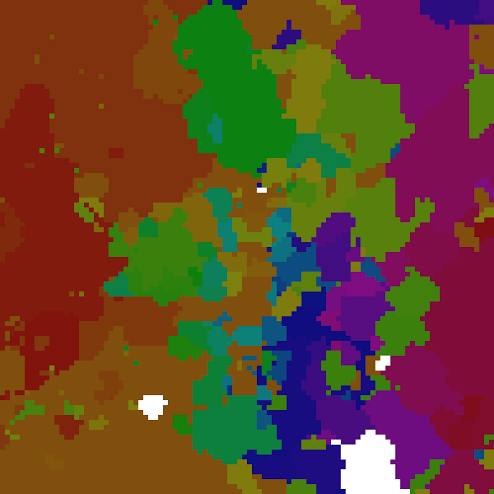
\includegraphics[scale=0.4]{monday.png}
\caption{}
\label{fig:patch_mon}
\end{figure}

\begin{figure}[h]
\centering
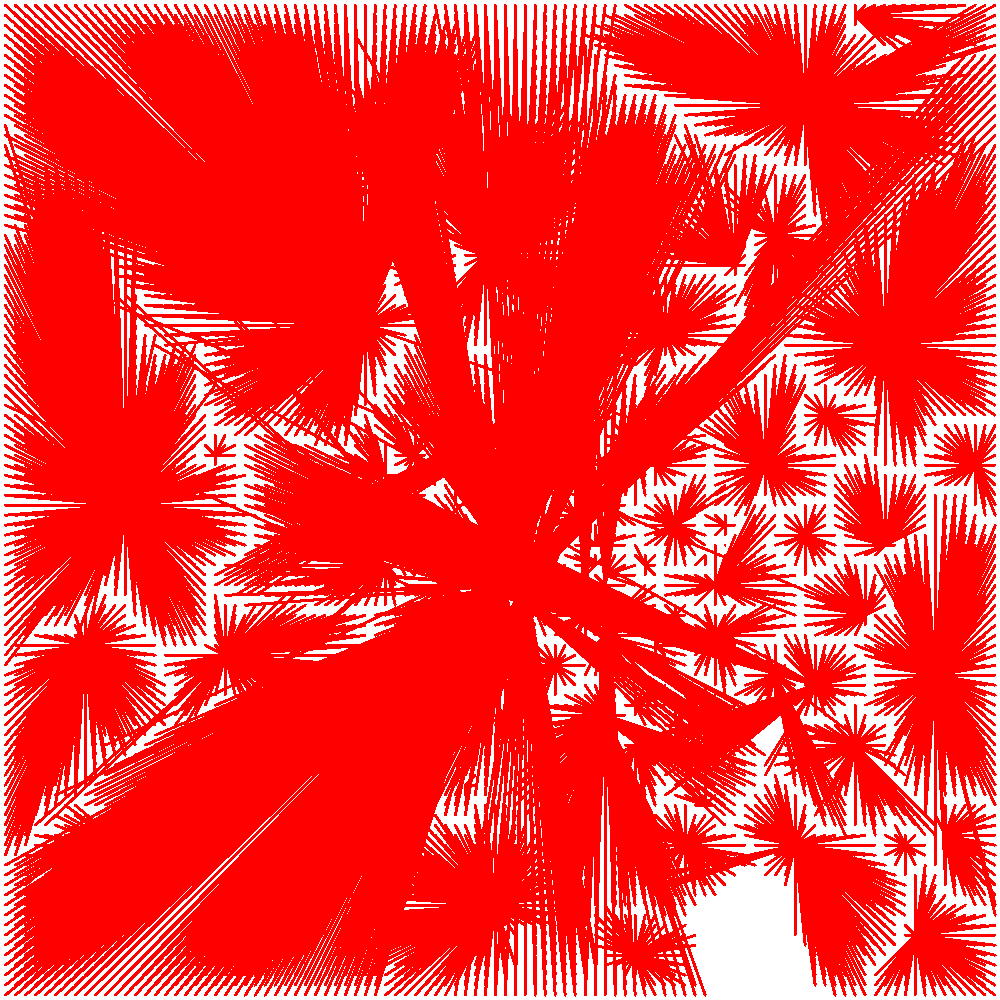
\includegraphics[scale=0.2]{clusters.png}
\caption{}
\label{fig:arcs_mon}
\end{figure}


\begin{figure}[h]
\centering
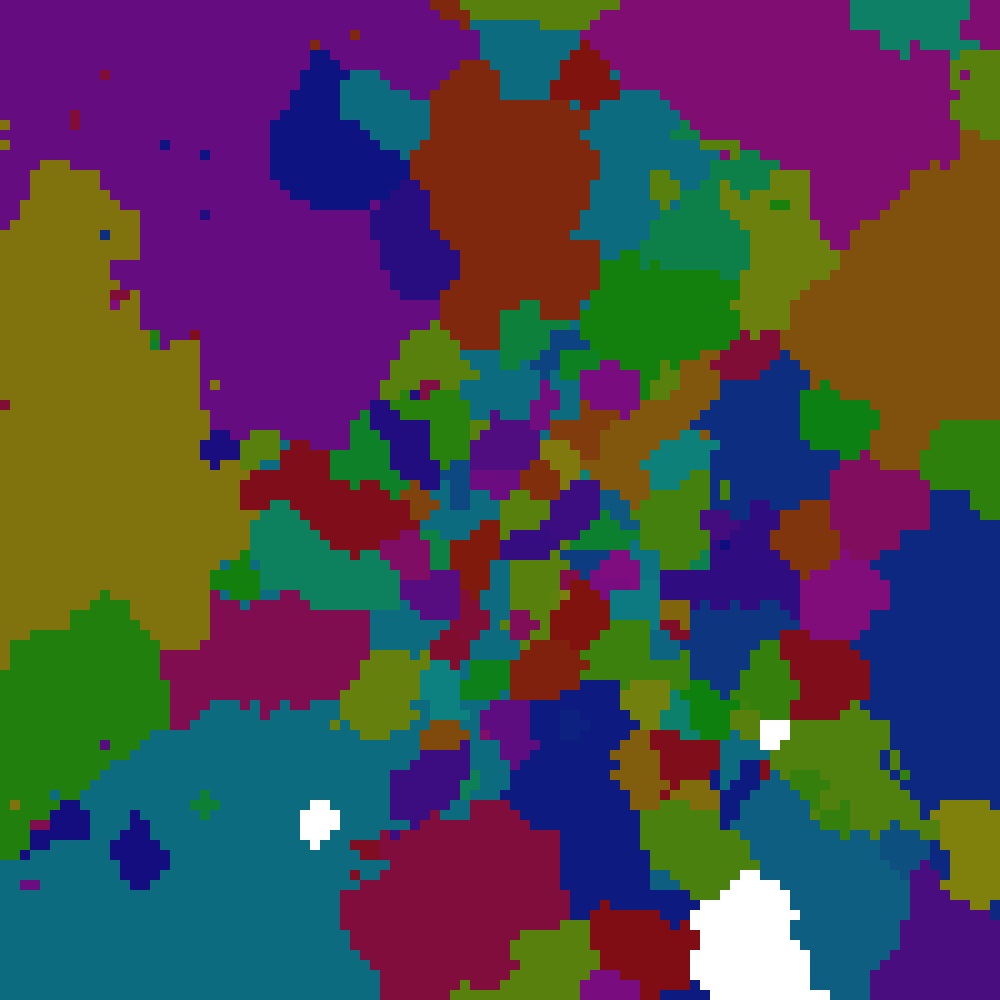
\includegraphics[scale=0.2]{wednesday.png}
\caption{}
\label{fig:patch_wed}
\end{figure}

\begin{figure}[h]
\centering
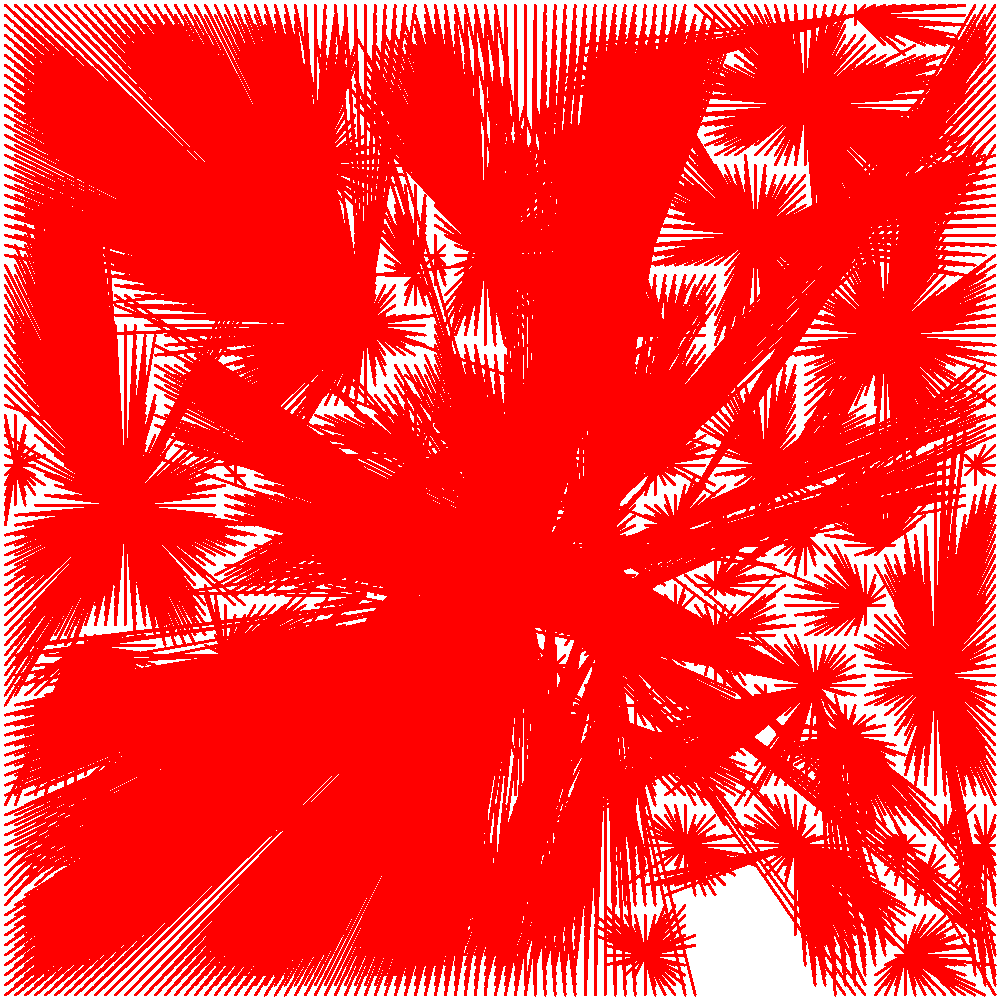
\includegraphics[scale=0.2]{wednesday_arcs.png}
\caption{}
\label{fig:arcs_wed}
\end{figure}


\end{document}
